




\section{Automatic Discrete Prompt Optimization}
\begin{algorithm}
\caption{Discrete prompt optimization: \modelname}  
\label{alg:evo}
\begin{algorithmic}[1]
\Require {Initial prompts $P_0 = \{p_1, p_2, \dots, p_N\}$,  size of population $N$, a dev set $\mathcal D$, $f_{\mathcal D}(\cdot)$} denotes the score of a prompt on the desired LLM evaluated on $\mathcal D$, a pre-defined number of iterations $T$, carefully designed evolutionary operators to generate a new prompt $\text{Evo}(\cdot)$

\State \textbf{Initial evaluation scores}: $S_0\leftarrow\{s_i=f_\mathcal D(p_i)| i\in[1,N]\}$

\For{$t = 1$ to $T$}  
    \State \textbf{Selection}: select a certain number of prompts from current population as parent prompts $p_{r_1},\dots,p_{r_k}  \sim P_{t-1}$ 
    \State \textbf{Evolution}: generate a new prompt based on the selected parent prompts by leveraging LLM to perform evolutionary operators $p_i' \leftarrow \text{Evo}(p_{r_1},\dots,p_{r_k})$
    \State \textbf{Evaluation}: $s_i'\leftarrow f(p_i', \mathcal D)$
    \State \textbf{Update}: $P_t\leftarrow \{P_{t-1}, p_i'\}$ and $S_t\leftarrow \{S_{t-1}, s_i'\}$ based on the evaluation scores
\EndFor
\State \textbf{Return} the best prompt, $p^*$, among the final population $P_T$: $p^*\leftarrow argmax_{p \in P_T} f(p, \mathcal D)$

\end{algorithmic}
\end{algorithm} 
Current advanced LLMs are typically interacted via black-box APIs, while the gradients and parameters are inaccessible. Evolutionary algorithms (EAs) are derivative-free algorithms with exceptional accuracy and rapid convergence. Accordingly, we consider introducing EAs into discrete prompt optimization. However, to generate new candidate solutions, evolutionary operators typically edit the elements in current solutions independently, without considering the connections between them. This makes it challenging to apply evolutionary operators on discrete prompts, which require coherence and readability. To address this challenge, we propose a synergistic approach that connects the natural language processing expertise of LLMs with the optimization capabilities of EAs, called \modelname. 
Specifically, LLMs generate new candidate prompts based on evolutionary operators, while EAs guide the optimization process to find the optimal prompts.

In order to implement \modelname in practice, it is necessary to instantiate it with a specific algorithm of EAs. There are various types of EAs, and in this paper, we consider two widely used algorithms, including Genetic Algorithm (GA)~\citep{holland1975adaptation} and Differential Evolution (DE)~\citep{storn1997differential}. GA is among the most highly regarded evolutionary algorithms~\citep{holland1975adaptation,holland1992adaptation,mitchell1998introduction,mirjalili2020genetic} and DE has emerged as one of the most widely utilized algorithms for complex optimization challenges since its inception~\citep{storn1997differential,price2013differential,das2010differential,pant2020differential}. In the following, we will first outline the proposed \modelname, and then instantiate \modelname with GA and DE respectively.













\subsection{Framework of \modelname}












 





EAs typically start with an initial population of $N$ solutions (prompts in our setting), then iteratively generate new solutions using evolutionary operators (e.g., mutation and crossover) on the current population and update it based on a fitness
function. Following typical EAs, \modelname mainly contains three steps:
\begin{itemize}[leftmargin=*]
    \item \textbf{Initial population}: Contrary to most existing automatic prompt methods that neglect priori human knowledge, we apply available manual prompts as the initial population to leverage the wisdom of humans. 
    Besides, EAs typically start from random solutions, resulting in a diverse population and avoiding being trapped in a local optimum. Accordingly, we also introduce some prompts generated by LLMs~\citep{zhou2022large} into the initial population.
    \item  \textbf{Evolution}: In each iteration, \modelname uses LLMs as evolutionary operators to generate a new prompt based on several parent prompts selected from the current population. To accomplish this, we design steps of the \emph{mutation} and \emph{crossover} operators for each specific type of EAs, along with corresponding instructions to guide the LLMs in generating new prompts based on these steps.
    \item \textbf{Update}: We evaluate the generated candidate prompts on a development set and retain those with superior performance, similar to the survival of the fittest in nature. The specific updating strategy may vary depending on the type of EAs used.
\end{itemize}
The algorithm stops when the number of iterations reaches a predefined value. The details of \modelname are outlined in Algorithm~\ref{alg:evo}. 
When instantiating \modelname with a specific algorithm of EAs, the evolutionary processes need to be adjusted, and the key challenge is to design the evolutionary operators on discrete prompts.







\begin{figure}
  \centering
    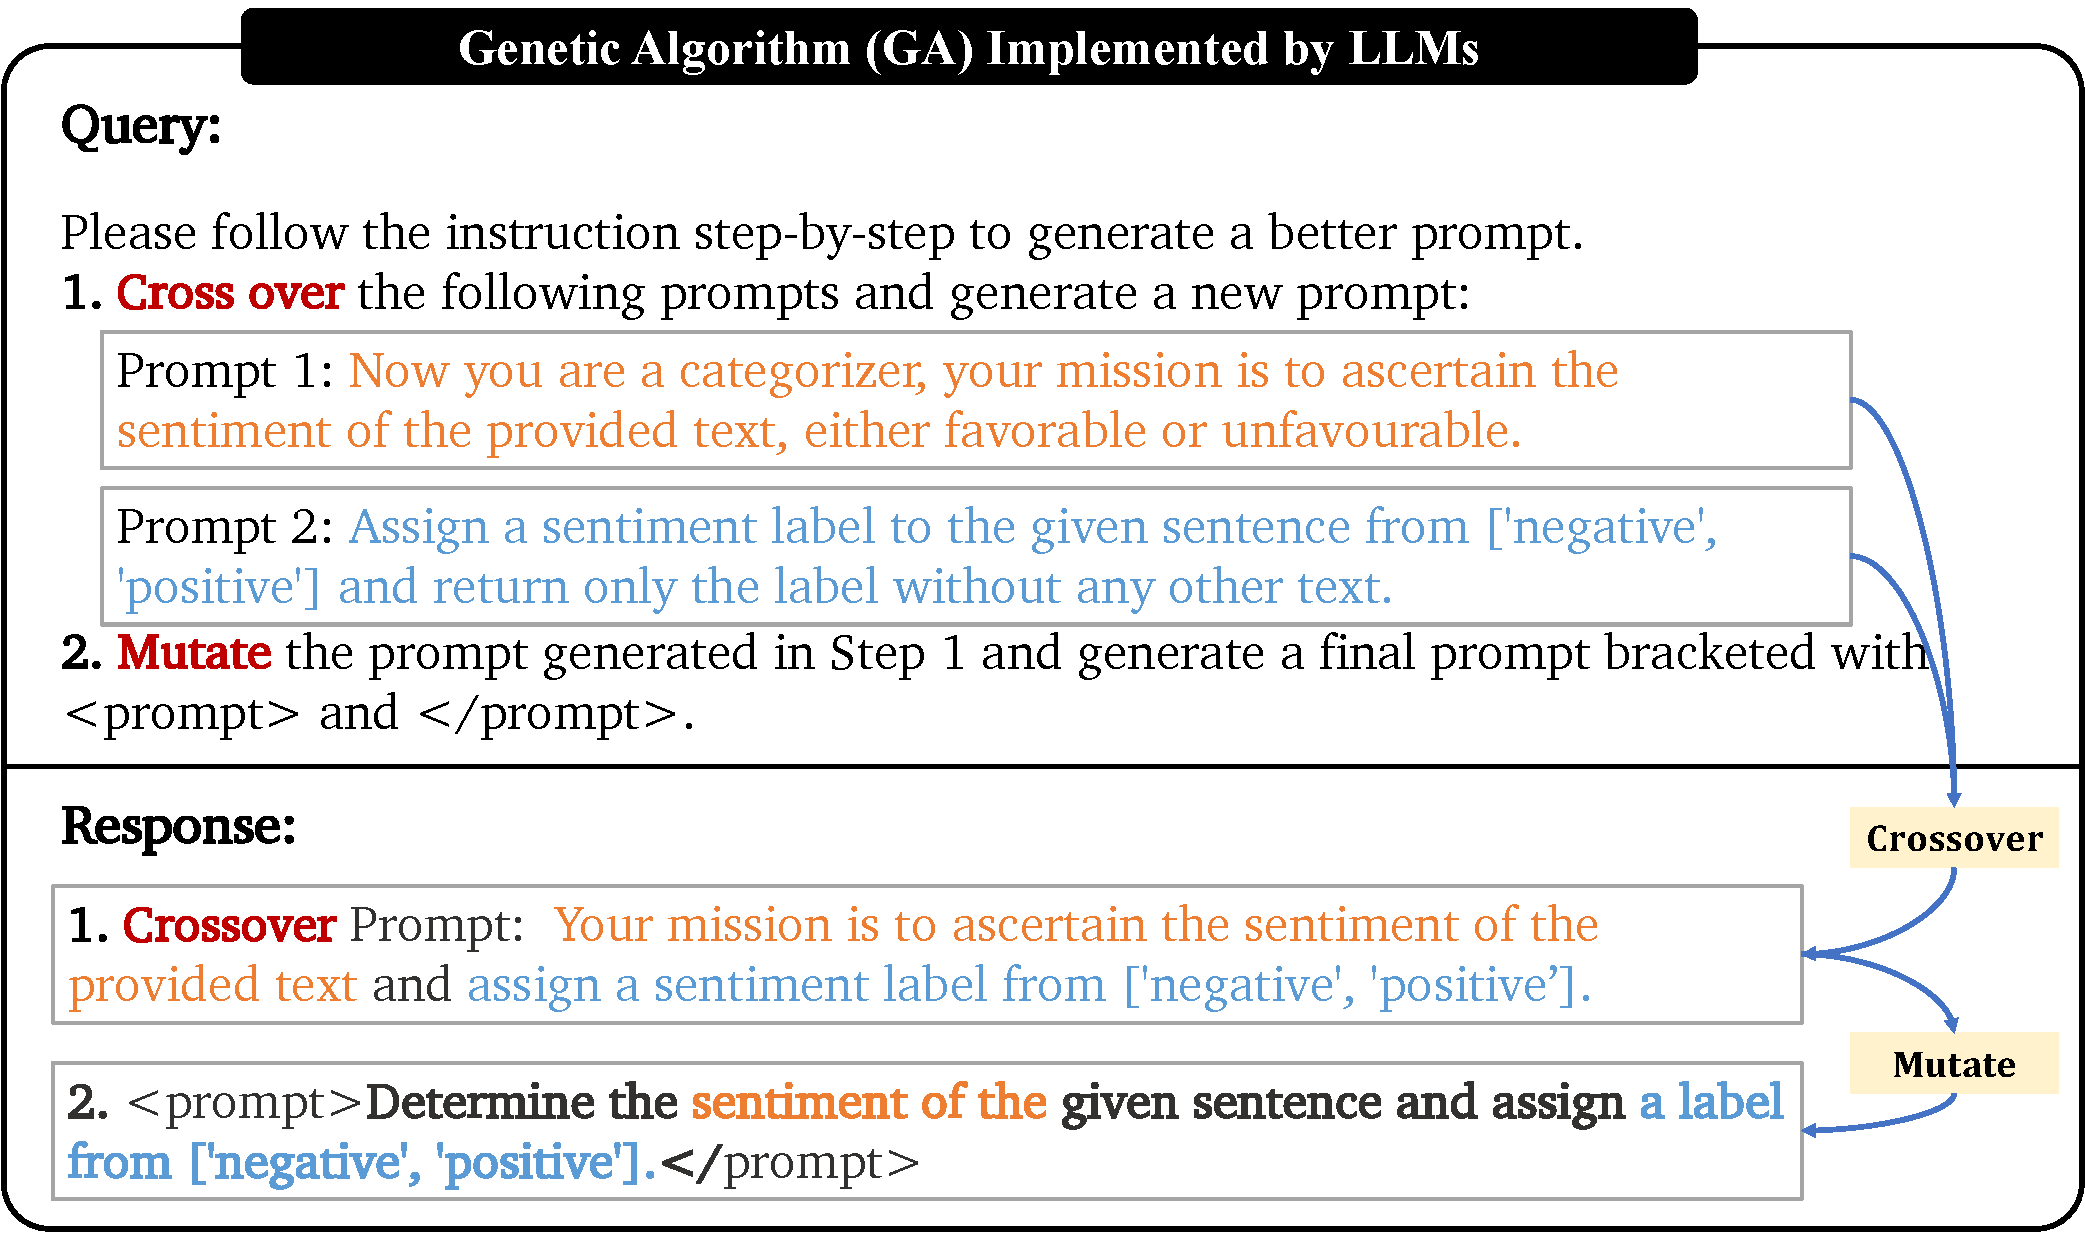
\includegraphics[scale=0.35]{images/ga_cot.pdf}
    \caption{GA process implemented by LLMs (Evo$(\cdot)$ in Algorithm~\ref{alg:evo}). In Step 1, LLMs perform \emph{crossover} on the given two prompts
    (words in \textcolor{Orange}{orange} and \textcolor{Blue}{blue} are inherited from Prompt 1 and Prompt 2, respectively). In Step 2, LLMs perform \emph{mutation} on the prompt. }

    \label{fig:ga_cot}
\end{figure} 
\subsection{Instantiation with Genetic Algorithm}
\paragraph{Selection} In GA, parent solutions are conventionally selected using the roulette wheel selection method, guided by their fitness values~\citep{lipowski2012roulette}. Analogously, we employ the roulette wheel selection to choose two parent prompts from the current population, based on their performance scores obtained on the development sets. Let $s_i$ denote the performance score of the $i$-th prompt within a population containing $N$ prompts.
The probability of selecting the $i$-th prompt as a parent can be expressed as ${p_i} = s_i/\sum_{j=1}^{N} s_j$.
 \begin{figure}
  \centering
    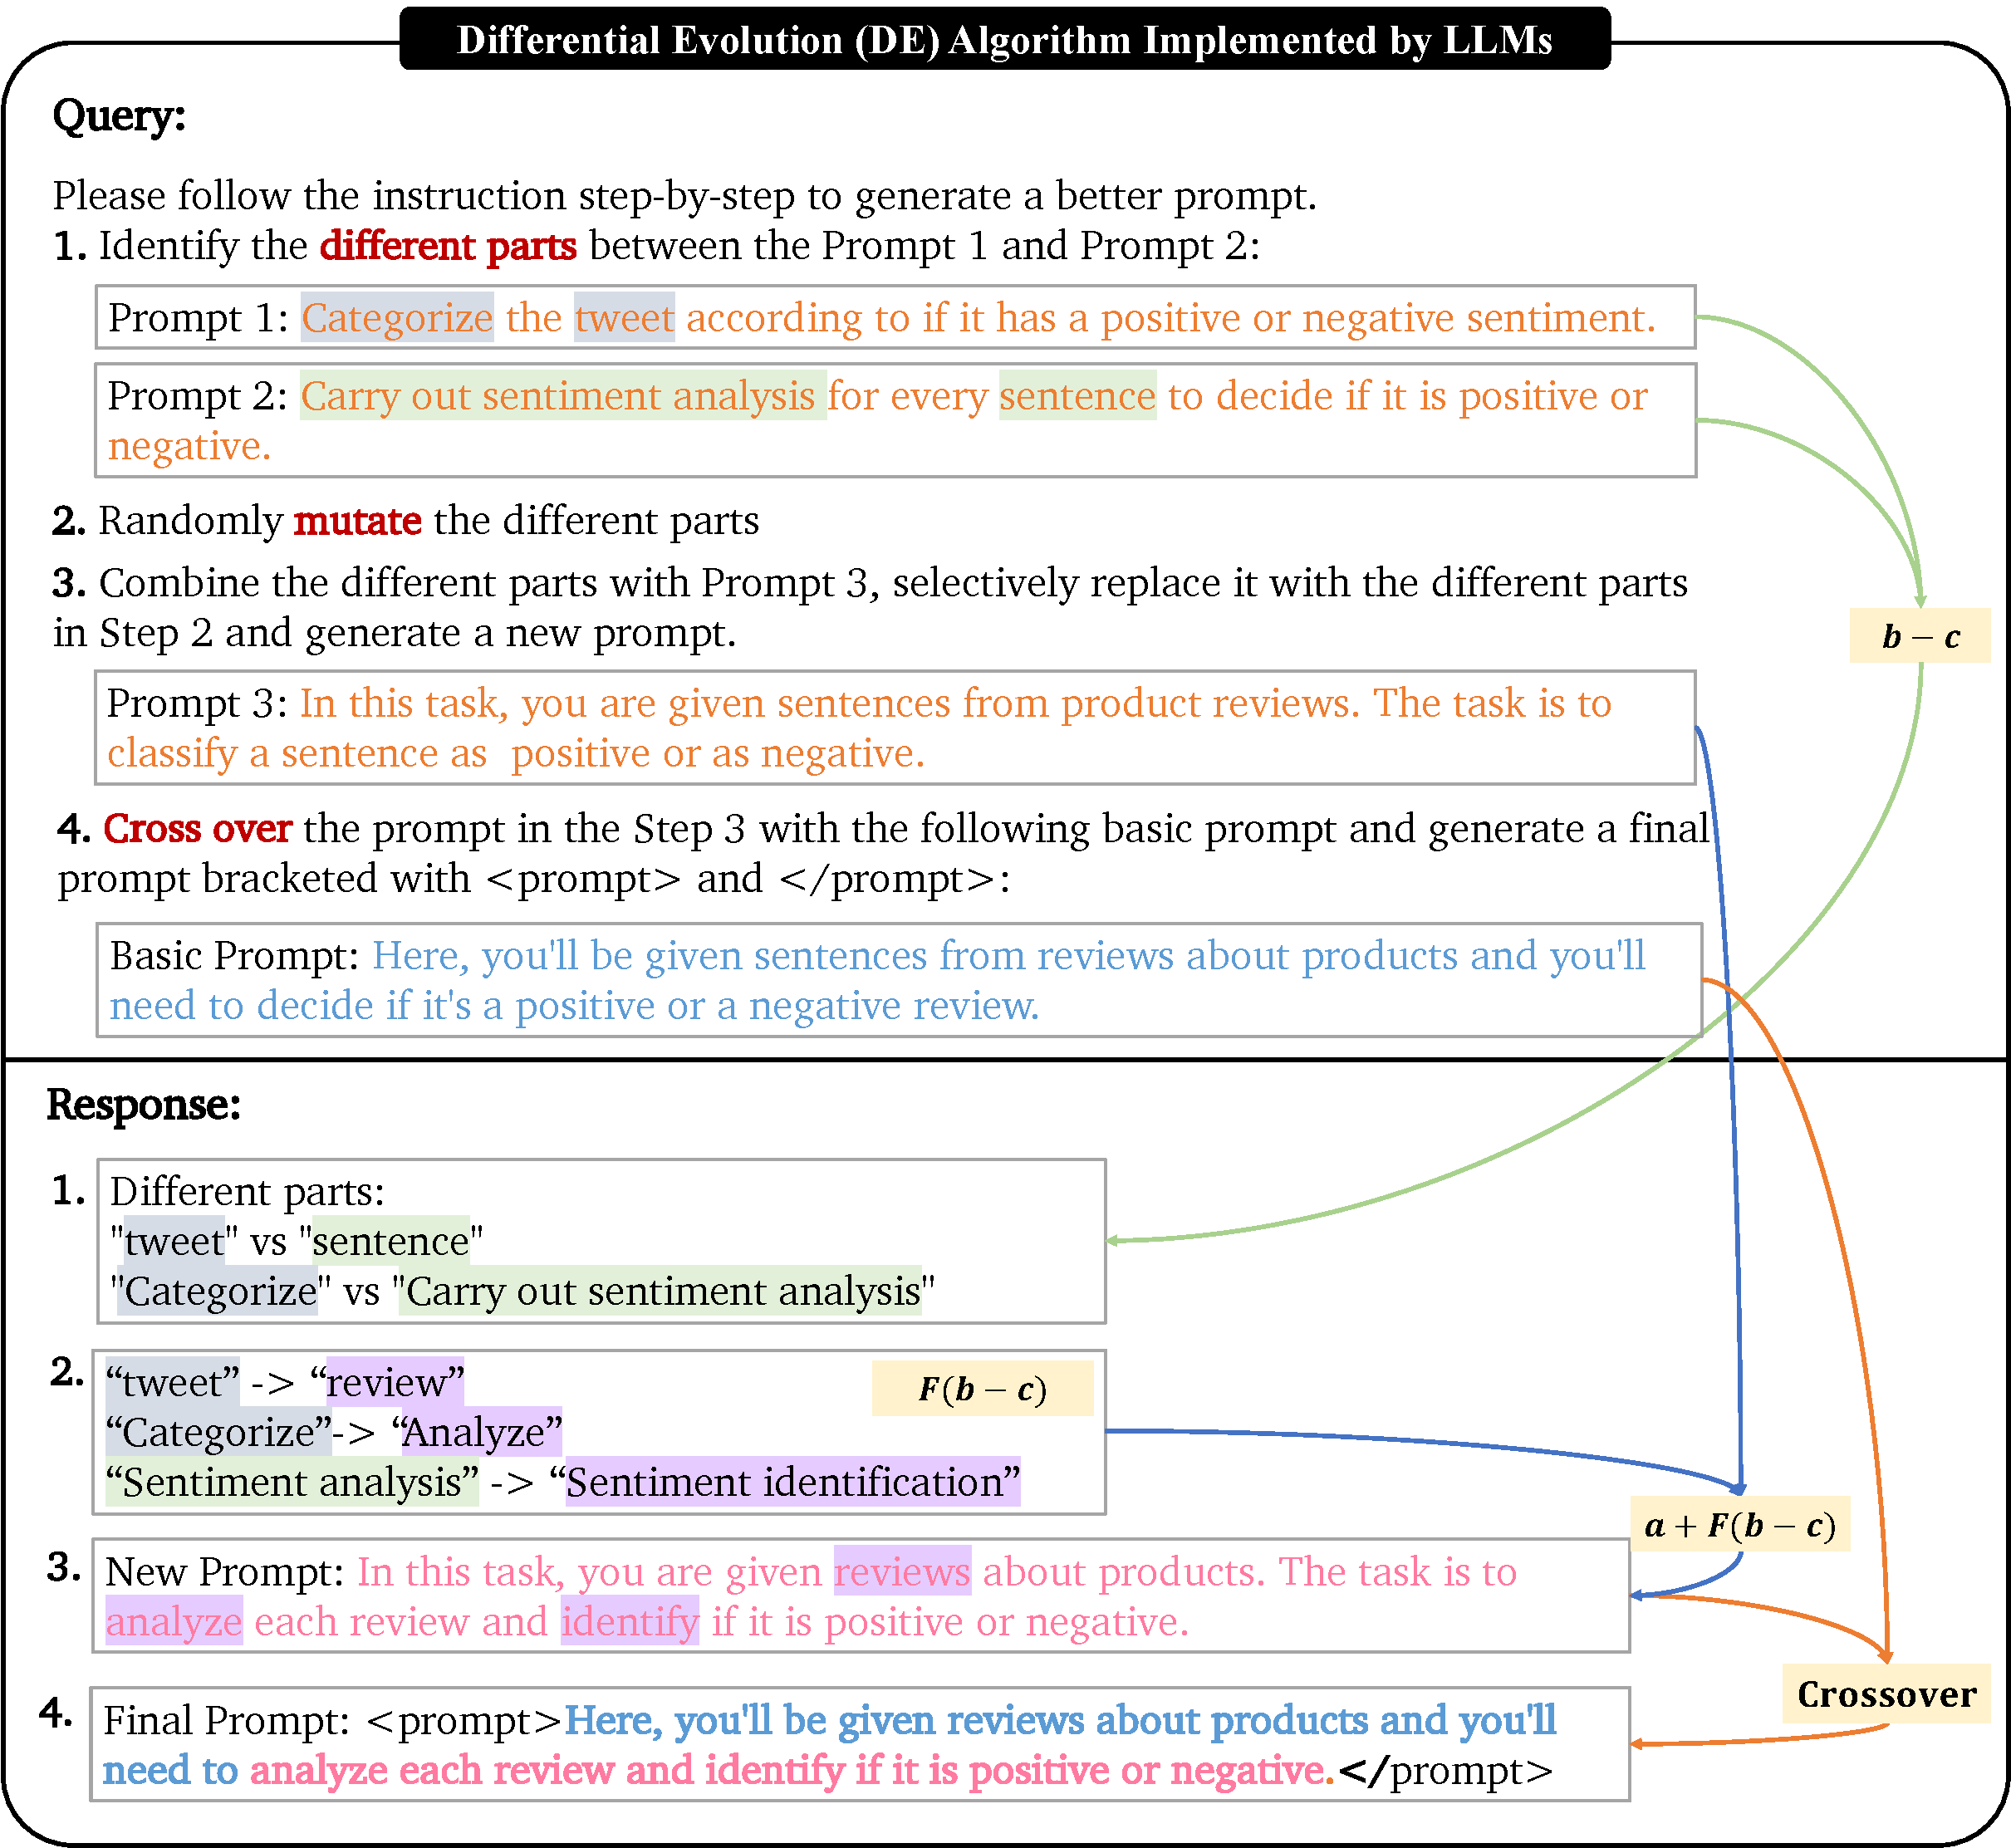
\includegraphics[scale=0.3]{images/de_cot_v2.pdf}
    \caption{DE process implemented by LLMs (Evo$(\cdot)$ in Algorithm~\ref{alg:evo}).
    In Step 1, LLMs find the different parts (words in \graybox\ and \greenbox) between \textcolor{Orange}{Prompt 1} and \textcolor{Orange}{Prompt 2} ($\mathbf{b-c}$ in typical DE). In Step 2, LLMs perform \emph{mutation} (words in \purplebox\ ) on them (imitation of $\mathbf{F(b-c)}$). Next, LLMs incorporate the \textcolor{Orange}{current best prompt} as \textcolor{Orange}{Prompt 3} with the mutated results in Step 2, to generate a new prompt (counterpart of $\mathbf{a+F(b-c)}$ in DE). Finally, LLMs perform \emph{crossover} upon the \textcolor{Blue}{current basic prompt} $p_i$ and the \textcolor{Pink}{generated prompt} in Step 3. See Figure~\ref{fig:de-cot-com} in Appendix~\ref{app:temp} for the complete response. }
    \label{fig:de_cot}
\end{figure}

\paragraph{Evolution} Conforming to the GA framework, we generate a new candidate prompt via two steps: \textbf{1)} Crossover is performed between the parent prompts to produce a new offspring prompt that inherits characteristics from both parents; \textbf{2)} Mutation is applied to the offspring prompt, introducing random alterations to certain elements. We formalize this two-stage operation into algorithmic instructions for guiding LLMs to implement $\text{Evo}(\cdot)$ in Algorithm~\ref{alg:evo}. The entire process is illustrated in Figure~\ref{fig:ga_cot}.



\paragraph{Update} We employ a straightforward selection strategy for updating the population: at each iteration, \modelname produces $N$ new prompts, which are merged with the existing population of $N$ prompts. Subsequently, the top $N$ prompts, based on their scores, are retained to form the updated population. Accordingly, the overall quality of the population undergoes continuous enhancement, culminating in the selection of the best one within the final population as the optimal prompt.

\subsection{Instantiation with Differential Evolution}

Here, we begin with some preliminary knowledge of DE. Unlike GA, the solutions of DE are represented by numerical vectors. Each vector within the population is sequentially selected as a base vector, denoted as $\mathbf{x}$, which subsequently undergoes mutation and crossover. 
During mutation, a mutated solution $\mathbf{y}$ is generated from a randomly selected solution $\mathbf{a}$ from the current population. The mutation is achieved by adding a scaled difference between two distinct, randomly selected solutions $\mathbf{b}$ and $\mathbf{c}$ to $\mathbf{a}$, i.e., $\mathbf{y} = \mathbf{a} + F(\mathbf{b} - \mathbf{c})$, where $F$ is the scaled parameter.

Crossover is to generate a trial solution $\mathbf{x'} = [x'_1,...,x'_n]$ by choosing each parameter in the vector from either the basic solution $\mathbf{x}$ or the mutated solution $\mathbf{y}$.
Then, $\mathbf{x}$ is replaced with $\mathbf{x'}$ if $\mathbf{x'}$ is better than $\mathbf{x}$. 
Within step-by-step evolution, DE ends with a population of high quality. A modified version of DE uses the current best solution as vector $\mathbf{a}$ to exploit information from the best one.

\paragraph{Evolution} The evolutionary process of DE can be decoupled into three steps: 1) $F(\mathbf{b} - \mathbf{c})$; 2) $\mathbf{y} = \mathbf{a} + F(\mathbf{b} - \mathbf{c})$; 3) Crossover of $\mathbf{x}$ and $\mathbf{y}$. In \modelname based on DE, we follow the three steps to design the evolutionary process, as well as the corresponding instructions for LLMs to generate a new prompt based on these steps as illustrated in Figure \ref{fig:de_cot}:
\begin{itemize}[leftmargin=*]
    \item Inspired by the differential vector in DE, we consider mutating only the different parts of two randomly selected prompts in the current population (Step 1 and Step 2 in Figure~\ref{fig:de_cot}). The prompts in the current population are considered the current best ones. Accordingly, the shared components of two prompts tend to have a positive impact on the performance, and thus need to be preserved.
    \item A variant of DE employs the current best vector during the mutation process, where a mutated vector is generated by adding the scale of the differential vector to the current best vector. Building upon this idea, we generate a mutated prompt by selectively replacing parts of the current best one with the mutated different parts for combination. (Step 3 in Figure~\ref{fig:de_cot}).
    \item Crossover replaces certain components of a basic prompt (i.e., a candidate of the current population) with segments from the mutated prompt. This operation combines the features of two different prompts, potentially creating a new and improved solution (Step 4 in Figure~\ref{fig:de_cot}).
\end{itemize}

\paragraph{Update} Following the standard DE, each prompt $p_i$ in the current population is chosen as a basic prompt in turn to generate a corresponding new prompt $p_i'$ using the instruction in Figure ~\ref{fig:de_cot}. Then, the prompt with a higher score, either $p_i$ or $p_i'$, is retained. Accordingly, the population size remains constant while the overall quality of the population is enhanced.


















